\documentclass{article}

\usepackage{arxiv}
\usepackage[utf8]{inputenc} 
\usepackage[T1]{fontenc}    
\usepackage{hyperref}      
\usepackage{url}            
\usepackage{booktabs}       
\usepackage{amsfonts}       
\usepackage{nicefrac}       
\usepackage{microtype}      
\usepackage{cleveref}       
\usepackage{graphicx}
\usepackage{natbib}
\usepackage{doi}
\usepackage[portuguese]{babel}
\usepackage{caption}
\usepackage{braket}
\usepackage{amsmath}


\newcommand{\tens}[1]{%
	\mathbin{\mathop{\otimes}\limits_{#1}}%
}


\title{Quantum Oracles - Como transformar problemas clássicos em quânticos}

\date{}


\author{ \href{https://orcid.org/0009-0008-9134-5974}{
\includegraphics[scale=0.06]{orcid.pdf}\hspace{1mm}Alexandre Silva}\\
	Ciências da Computação\\
	UNIVEM - Centro Universitário Eurípides de Marília\\
}

\graphicspath{ {../images/} }


\renewcommand{\headeright}{}
\renewcommand{\undertitle}{}
\renewcommand{\shorttitle}{}


\hypersetup{
	pdftitle={Quantum Oracles - Como transformar problemas classicos em quanticos},
	pdfsubject={quantum computing, computer science, ciencias da computacao, computacao quantica, algoritmos, algorithms},
	pdfauthor={Alexandre Silva},
	pdfkeywords={quantum oracles, quantum, quantum computing, algoritmos, algorithms},
}

\begin{document}
\maketitle
\begin{abstract}
	
\end{abstract}


\section{Introdução}
Hoje, não é difícil ver alguém falando sobre computação quântica e como essas máquinas vão mudar o futuro. Contudo, muitas dessas frases acabam se levando por extrapolações e/ou usos indevidos de ficção. Neste artigo, mostrarei que nem tudo é possível ser feito com um computador quântico atual, assim como existem pequenas áreas que se beneficiam ao máximo dessa nova tecnologia.\\
Para esse feito, serão mostrado alguns testes feitos usando o \href{https://www.ibm.com/quantum/qiskit}{qiskit}, um framework open source da IBM para computação quântica, além de alguns resultados obtidos após executar os algoritmos em simuladores e máquinas reais, assim como seus relativos em computação clássica. Algoritmos dos quais tomam proveito dos quantum oracles, modelos ideias de função que não ajudam a descrever o algoritmo matematicamente, também tomam proveito de alguns efeitos quânticos, como superposição e interferência, para se sobressair à algumas estratégias clássicas.\\
Com isso, o projeto foi desenvolvido em cima de cinco pequenos problemas, sendo eles: conversão de milhas para quilômetros, torre de Hanoi, explorador de arquivos, Buckshot Roulette e QRAM. Todas as implementações e materiais utilizados podem ser encontrados \href{https://github.com/Dpbm/scientific-initiation-1-quantum-oracles}{nesse repositório do GitHub}.


\section{Início do projeto}
Para dar início a pesquisa, foi necessário entender quais os tipos de oracles existem e como eles podem ser usados.\\
Em computação clássica, temos as Oracle Machines, as quais são maquinas de Turing, das quais implementam alguma função em seu interior, e ao ser chamado/invocado o resultado correto é retornado em tempo constante $O(1)$, podendo ser vista como uma caixa preta, abstraindo completamente o seu funcionamento. Devido a essa definição, as OMs são ideias matemáticos, sendo assim usados apenas para formalismo matemático.\\
Contudo em computação quântica, podemos de fato implementar certos modelos de Oracles e adiciona-los a um circuito maior, executando certas funções como: encoding de dados, aplicação de $f(x)$, abstração de partes do circuito, etc.

\subsection{Tipos de Oracles}

\subsubsection{Phase Oracle}
Um dos primeiros tipos de Oracles usados para a criação de algoritmos como os de: \href{https://en.wikipedia.org/wiki/Grover%27s_algorithm}{Grover} e \href{https://en.wikipedia.org/wiki/Deutsch%E2%80%93Jozsa_algorithm}{Deutsch–Jozsa}; é comummente conhecido como \emph{Phase Oracle}.\\
Tal dispositivo, é usado para atribuir uma fase ao circuito, sendo muito usado para configurar valores, explorar a interferência ou se aproveitar de outros efeitos como o \textit{Phase Kickback}. Matematicamente poderiamos descrever ele da seguinte forma: $\ket{x}\ket{-} \to (-1)^{f(x)}\ket{x}\ket{-}$, do qual $\ket{x}$ é a entrada do oracle e $\ket{-}$ é a ancilla que prove a fase.

\begin{center}
	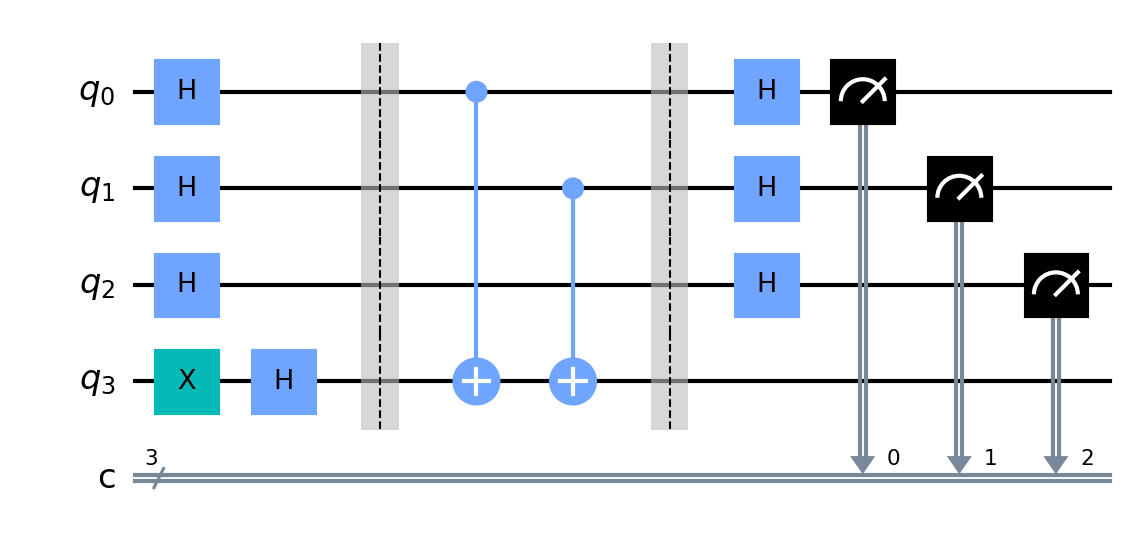
\includegraphics[scale=0.3]{phase_oracle_1.png}
	\captionof{figure}{Exemplo de phase oracle usado para o algoritmo de Deutsch–Jozsa}
	\label{fig:phase-oracle-1}
\end{center}

No exemplo acima, utilizamos o \textit{Phase Kickback} para adicionar uma fase nos qubits 0 e 1, transformando seus estados de $\ket{+}$ para $\ket{-}$, fazendo com que ao serem colapsados o resultado $\ket{1}$ apareça na saída.\\

É possível também criar um phase oracle removendo o qubit adicional (nesse exemplo o Q3), uma vez que podemos utilizar outros gates para introduzir a fase e manter ainda natureza unitária.

\begin{center}
	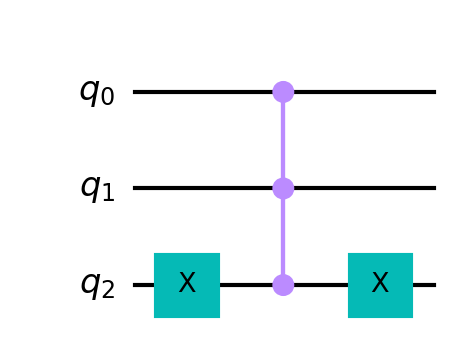
\includegraphics[scale=0.3]{phase_oracle_2.png}
	\captionof{figure}{Exemplo fase Oracle sem a Ancilla}
	\label{fig:phase-oracle-2}
\end{center}


Dessa vez, utilizamos o $MCP$ gate para adicionar uma fase global $\pi$ e dois gates $X$ para dizer quais qubits queremos q tenham o valor 0, codificando assim o valor $011$ ou $3$ na base decimal.

\begin{center}
	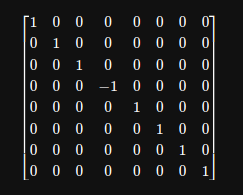
\includegraphics[scale=0.5]{phase_oracle_unitary.png}
	\captionof{figure}{Matriz unitária do Phase oracle}
	\label{fig:phase-oracle-unitary}
\end{center}

É possível verificar então que ao criarmos esse circuito, matemos a matriz identidade e adicionamos a fase $-1$ no valor da coluna relativa ao $011$. \\
Essa versão pode ser considerada como um minimal oracle, uma vez que a própria função interna se mantém unitária, sem a necessidade de ancilla.


\subsection{Boolean Oracle}

O Boolean oracle, por sua vez, representa uma função booleana, sem qualquer adição de fases.\\
Nesse caso, $\ket{x}$ representa a entrada do oracle e $\ket{y}$ represetam os qubits auxiliares que receberam a resposta, $\ket{x}\ket{y} \to \ket{x}\ket{y \oplus f(x)}$.

\subsection{Minimal oracle}

Como já citado anteriormente, o minimal oracle possui uma função que em sua essência é unitária, não requerendo qubits adicionais $\ket{x} \to \ket{f(x)}$.

\begin{center}
	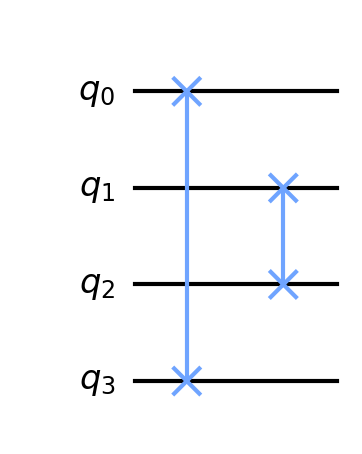
\includegraphics[scale=0.3]{minimal-oracle.png}
	\captionof{figure}{Exemplo de minimal oracle}
	\label{fig:minimal-oracle}
\end{center}

Lembrando que este pode também adicionar fases ao circuito.

\subsection{Simon's Oracle}

O Oracle de Simon, é uma instância do Boolean Oracle. Neste visamos encontrar os períodos da função implementada, ou seja, dado $x$ e $f(x) = y$ existe ao menos uma função em que $f(y) = x$ ?


\begin{center}
	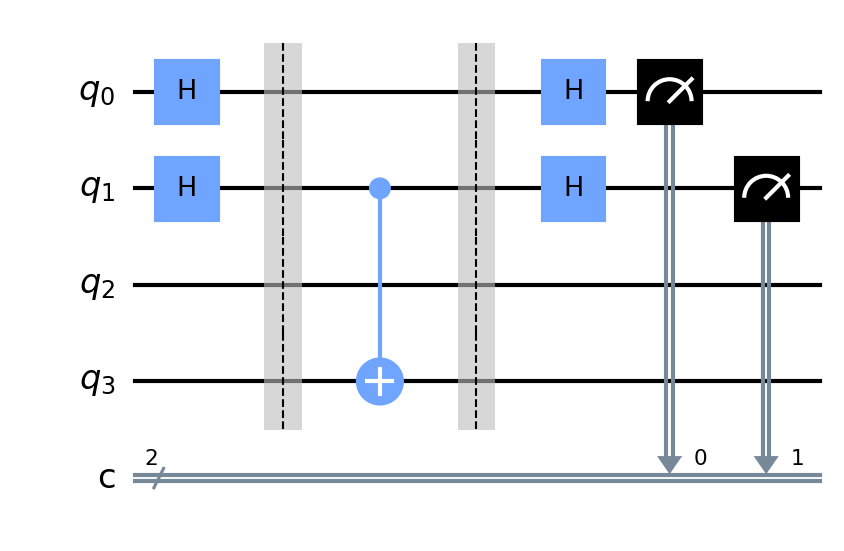
\includegraphics[scale=0.3]{simons.png}
	\captionof{figure}{Exemplo do algoritmo de Simon}
	\label{fig:simons-oracle}
\end{center}

Nesse algoritmo, configuramos uma chave $s$ dentro do oracle, e ao executar o algoritmo temos os possíveis períodos da função, sendo necessário rotinas de pós processamento para identificar o valor correto.

\subsection{QFT(Quantum Fourier Transformation) Oracle}

Por fim, o Oracle QFT aplica a versão quântica da transformada de Fourier, projetando os valores de entrada na base $X$ (também conhecido como base de Fourier).


\begin{center}
	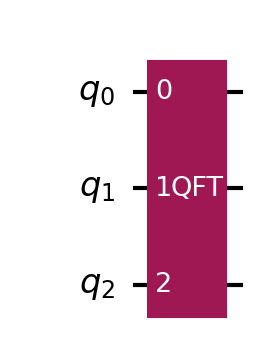
\includegraphics[scale=0.4]{QFT_1.png}
	\captionof{figure}{Exemplo do algoritmo de QFT}
	\label{fig:QFT}
\end{center}

\begin{center}
	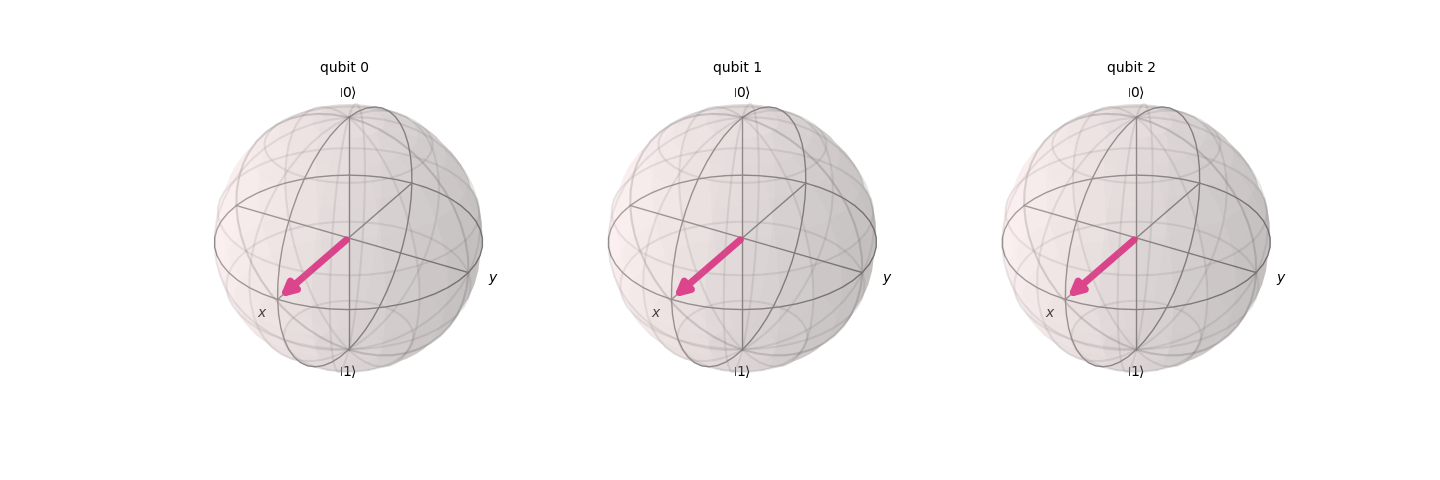
\includegraphics[scale=0.3]{QFT_1_bloch.png}
	\captionof{figure}{Valores mapeados na base de Fourier}
	\label{fig:QFT-bloch}
\end{center}


\section{Desenvolvimento}
\subsection{File Explorer}

Imagine um computador quântico com um sistema operacional quântico (semelhante aos computadores convencionais, mas dessa vez seguindo as leis da mecânica quântica). Pensando nas partes desse sistema operacional, como seria possível pegar arquivos da memória usando a computação quântica?


\subsubsection{Algoritmos usados}

\subsubsection{Grover}
Um dos algoritmos mais comuns para a área é o algoritmo de Grover. Esse algoritmo realiza buscas em "bancos de dados"(bit strings) desorganizados em tempo $O(\sqrt{2^n})$ onde $n$ é o número de qubits usados. Nele, usamos um circuito do qual amplifica-se a probabilidade de encontrar os valores marcados no Oracle na saída.
Tal algoritmo segue o seguinte padrão: \
\begin{enumerate}
	\item{Configuramos todas as possíveis bit strings, ou seja aplicamos uma superposição uniforme $H^{\tens{^n}}$}
	\item{aplicamos o phase oracle $Uf$ do qual implementa uma função que marca os valores que desejamos encontrar}
	\item{aplicamos o operador de Grover Diffuser, $\mathbb{I} - 2 \ket{s}\bra{s}$}, sendo $s$ o estado com o valor que queremos
\end{enumerate}

Convertendo para um circuito temos algo semelhante a:


\begin{center}
	\includegraphics[scale=0.3]{Grover.png}
	\captionof{figure}{Exemplo algoritmo de Grover}
	\label{fig:grover-default-circuit}
\end{center}

Para 1 ou 2 valores, podemos usar a configuração acima. Mas maiores quantidade de valores, precisamos adcionar o conjunto Oracle + Diffuser $k$ vezes, sendo $k \approx { {\pi \over {4 \sqrt{a\over{2^n}}}} - {1\over2}  }$, sendo $a$ o numero de valores marcados.

\subsubsection{Diferença de conjuntos}

Utilizando os phase oracles, podemos criar dois Oracles distintis com ranges de valores diferentes e sobrepor seus valores, realizando a operação de diferença de conjuntos.

\begin{center}
	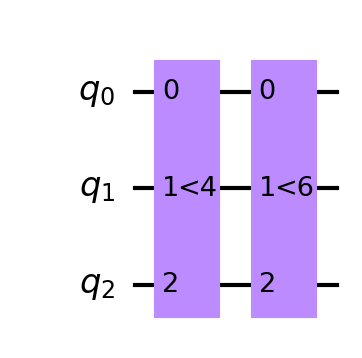
\includegraphics[scale=0.3]{less_than.png}
	\captionof{figure}{Exemplo de diferença de conjuntos}
	\label{fig:less-than-circuit}
\end{center}

Nesse exemplo foi encodado no primeiro oracle o set $\{000, 001, 010, 0110\}$ e no segundo $\{000, 001, 010, 011, 100, 101\}$.

\begin{center}
	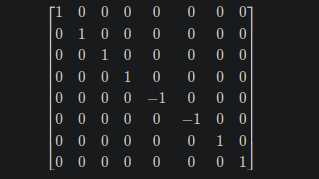
\includegraphics[scale=0.5]{less_than_unitary.png}
	\captionof{figure}{Resultado da diferença de conjuntos}
	\label{fig:less-than-circuit-unitary}
\end{center}

Como pode ser visto, apenas os valores $\{100, 101\}$ permaneceram com a fase, representando então a sobreposição delas.


\subsubsection{Solução para o problema}

Para a solução do problema, podemos criar em uma hash function $C(v)$ da qual recebe o path de um arquivo e retorna uma bit string respectiva. Com essa função em mãos, podemos utilizar o conjunto dos valores retornados e encoda-los em um phase oracle, agindo como uma especie de Look Up Table para os arquivos existentes na máquina.

No entando, para ter sucesso na pesquisa, é necessário utilizar um segundo Oracle encondando $S = P-s$, sendo $s$ o conjunto de arquivos do qual estamos procurando e $S$ os arquivos restantes, aproveitando-se então da diferença de conjuntos para encontrar então apenas os valores desejados para a pesquisa.


\begin{center}
	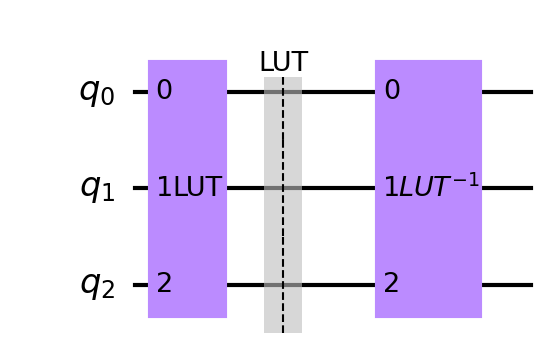
\includegraphics[scale=0.6]{sets-difference-look-up-table-oracle.png}
	\captionof{figure}{Diferença de conjuntos com as Look Up Tables}
	\label{fig:luts}
\end{center}

Sendo assim, o primeiro oracle age como o HD da marquina, marcando todos os arquivos existentes, e o segundo age como o mediador da pesquisa.

Com isso, adicionamos a Look Up Table final ao algoritmo de Grover.

\begin{center}
	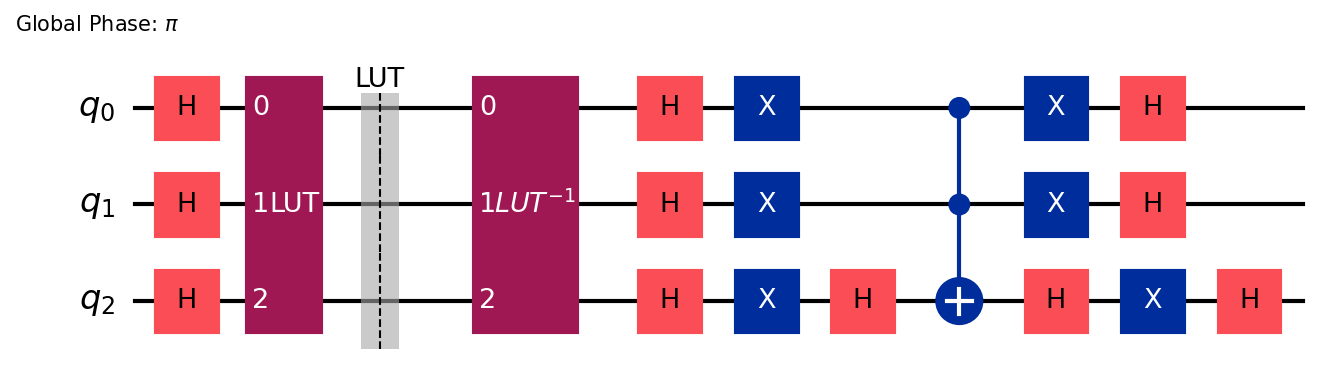
\includegraphics[scale=0.5]{file_explorer.png}
	\captionof{figure}{File explorer circuito}
	\label{fig:file-explorer}
\end{center}

\subsubsection{Resultados}

Para um caso hipotetico de sistema completamente quântico, certamente esse é um das maneiras de encontrar arquivos em meio a todos os outros.

Contudo, como o objetivo dessa pesquisa sugere, para utilizar esse modelo em um sistema clássico tomando proveito da computação quântica, não se mostra como a melhor opção.

Para sistemas convencionais, dos quais utilizam métodos baseados em árvores, não é possivel tirar qualquer proveito aqui, sendo $O$ polinomial contra $O$ quadrático.

Mesmo perante os testes clássicos feitos durante o desenvolvimento, esse protocolo só se mantém util quando a pesquisa era feita de forma linear.


\begin{center}
	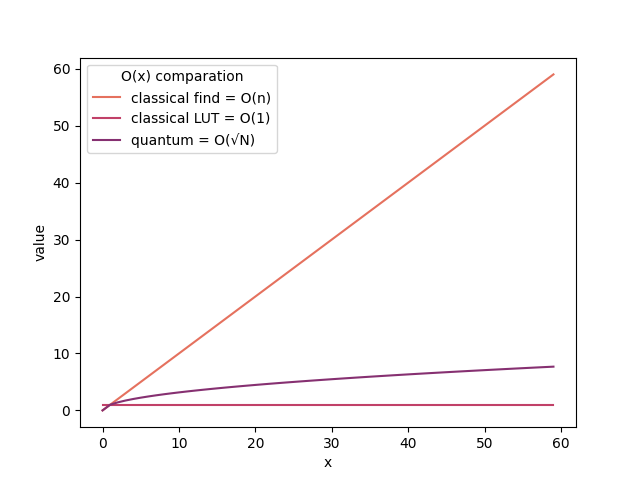
\includegraphics[scale=0.5]{algorithms-finding-comparation.png}
	\captionof{figure}{Comparação algoritmos usados na pesquisa}
	\label{fig:file-explorer-comparation-O}
\end{center}

Sendo assim, o algoritmo de Grover deve ser pensando para casos do qual a versão clássica possui complexidade $\ge O(n)$.


\subsection{Miles to Kilometers}
\subsection{Hanoi Tower}
\subsection{Buckshot Roulette}
\subsection{QRAM}

\begin{center}
\end{center}

\nocite{SOARE2009368}
\nocite{odonnell_2015_lecture}
\nocite{bacon_2006_cse}
\nocite{lipics_stacs}
\nocite{odonnell_2015_lecture_2}
\nocite{brodkorb_2019_the}
\nocite{amreen_oracle}
\nocite{kalyanasyndaram_2021_mod04lec23}
\nocite{davis_2006_turing}
\nocite{viswanathan_2013_reductions}
\nocite{Fan_2007}
\nocite{cryptoeprint:2020/1270}
\nocite{buhrman1998quantum}
\nocite{sanchezrivero2023initial}
\nocite{gilliam2020canonical}
\nocite{Kashefi_2002}
\nocite{e21080800}
\nocite{Zeng_2014}
\nocite{atici2004comparative}
\nocite{sundarappan_2022_how}
\nocite{dai_view}
\nocite{sep-game-theory}
\nocite{Giovannetti_2008}
\nocite{jaques2023qram}
\nocite{PythonEWL2022}
\nocite{frackiewicz2011application}
\nocite{Eisert_1999}
\nocite{usman_2019_kilometres}
\nocite{ldiaandr_2021_tower}
\nocite{diptokarmakar47_2019_how}
\nocite{a2020_towers}
\nocite{geeksforgeeks_2014_program}
\nocite{khan_2021_quantum}
\nocite{legn_2022_dilemma}
\nocite{siegelwax_2022_quantum}
\nocite{landi_density}
\nocite{bacon_2006_cse}
\nocite{vijayakrishnan_2019_role}
\nocite{python_scientific}
\nocite{scipyoptimizeminimize_scalar}
\nocite{davis_optimization}
\nocite{scipyoptimizeminimize}



\bibliographystyle{unsrt}
\bibliography{references}


\end{document}
